\section{Introduction}
\label{sec:introduction}

Set up SMAC, what we did with it, and what we learned.

\todo{The following could be moved to Background if we think it makes more
	sense there.}
It is important to keep in mind that there is little in this paper that is
specific to SMAC or its details or, for that matter, Clojush or its details. 
There are many approaches to parameter
tuning, and presumably similar results could have been acquired with many of
them. What matters the most here is that:
\begin{itemize}
	\item SMAC was able to discover parameter settings that 
	\emph{substantially} improved the performance
	of Clojush on the Replace-space-with-newline problem.
	\item Applying those optimized parameter settings to a variety of other
	problems let to very mixed results, suggesting that those parameter
	settings were very specific to the particular problem used for the SMAC
	search.
\end{itemize}
The fact that SMAC was able to discover settings that improved
performance on the Replace-space-with-newline problem by such a wide margin
is quite impressive. The fact that those parameter settings don't appear to
generalize is in no way the ``fault'' of SMAC, and are likely much more 
about how we used the tool than any property of the tool itself.

\section{Background}
\label{sec:background}

\begin{itemize}
	\item The citation the SMAC people ask us to use is~\cite{HutHooLey11-SMAC}.
	\item We should also probably cite their GECCO 2013 
	paper~\cite{hutter2013evaluation} as a prior example of using this in EC.
\end{itemize}

This is pretty fuzzy to me (Nic). We don't need to say a lot about \emph{how}
SMAC works, but we do need to talk about \emph{what it does}. Maybe that just
gets blended into the introduction?

Somewhere we'll presumably need to acknowledge that (a) there's been lots of
work historically on parameter optimization (e.g., early work on things like
population sizes and mutation rates in GAs) and (b) SMAC is by no means the
only tool of its kind out there. It would be great if someone could do some
lit review on that latter question in particular. (A few early examples would
be sufficient to make the first point; the latter is more politically charged.)

We also need to provide at least a minimal overview of Push/Plush/Clojush so
we can explain the meaning/action of the the parameters we chose to tune. 

\section{Tuning parameters for Replace-space-with-newline}
\label{sec:tuningRSWN}

% Describe the August work in Morris.

\todo{The following is almost certainly overly chatty and historical (vs.
	scientific), and will probably need to be cleaned up. It's just how
	I find myself thinking about it, and it seemed better to write *something*
	than sweat those bullets right now. -- Nic}

After hearing about SMAC at Holger Hoos's keynote at GECCO in July, 2016, we
decided to see if we could use SMAC to optimize parameters for Clojush, a
Clojure implementation of PushGP. PushGP is a stack-based genetic programming
system that has been demonstrably successful on a wide range of software
synthesis problems~\cite{Helmuth:2015:GECCO}. Like most ``industrial
strength'' EAs, Clojush has dozens of parameters that need to be set by the
practicioner, ranging from ``standard'' parameters like the population size
and the maximum number of generations to more Push-specific parameters\todo{
	Are these \emph{Push}-specific, or \emph{Plush}-specific? Do we want to
	get into those weeds? Do we want/need to bring Plush into it at all?}
such as \emph{alignment deviation} and \emph{uniform close mutation} (described
in Section~\ref{sec:background} above).\todo{Which means we need to have actually described them up above.}

After some initial work to set SMAC up to work with Clojush, and convince
ourselves that SMAC was in fact likely to perform some useful parameter
optimization, we set up three extended SMAC runs, each working independently
to optimize parameters for the Replace-space-with-newline software synthesis 
problem.\todo{Do we need to describe RSWN? The other 4? Where? In the Background section?}
This optimization depended on two important sets of choices:
\begin{itemize}
	\item The parameters to be optimized, and over what ranges
	\item The settings applied to SMAC, such as how long to set it search
\end{itemize}
These will be described below, along with the results of that optimization.

\subsection{Parameters optimized}
\label{sec:parametersOptimized}

Clojush exposes dozens of parameters that could potentially be optimized, but
adding parameters effectively increases the dimensionality and size of the
search space SMAC is required to explore. Thus exposing every possible parameter
seemed unwise, especially in a first experiment with the tool. We chose then
to focus primarily on parameters that controlled the genetic operators, along
with the population size and the selection mechanism. The parameters we chose 
to explore, the ranges SMAC should explore for each parameter, and the 
default initial values, are all listed in Table~\ref{tab:clojushParameters}.
In each case the default initial value was the same value used for all the
experiments in~\cite{Helmuth:2015:GECCO}.

\begin{table}
	\begin{center}
	\begin{tabular}{l@{\quad} @{\enskip}l@{\quad} @{\enskip}r@{\quad} @{\enskip}l}
		Parameter & Range & Default & Modifiers \\
		\hline
		Population size & $[1, 30K]$ & 1,000 & integer, log \\
		% Maximum generations & $[1, 30K]$ & $30,000/\textrm{population size}$ \\
		Selection method & tournament or & lexicase & categorical \\
		& \quad lexicase \\
		\hline
		Alternation prob. & $[0, 1]$ & 0.2 \\
		Uniform mutation prob. & $[0, 1]$ & 0.2 \\
		Uniform close mutation prob. & $[0, 1]$ & 0.1 \\
		(Alternation, Uniform mutation) prob. & $[0, 1]$ & 0.5 \\
		\hline
		Alternation rate & $[0, 1]$ & 0.01 \\
		Alignment deviation & $[0, 400]$ & 10 & integer \\
		\hline
		Uniform mutation rate & $[0, 1]$ & 0.1
	\end{tabular}
	\end{center}
	\caption{Clojush parameters optimized by SMAC for the Replace-space-with-newline problem, along with their ranges, 
		default values, and modifiers. See Section~\ref{sec:parametersOptimized} for additional details.}
	\label{tab:clojushParameters}
\end{table}

\todo{Should ``Maximum generations'' be in the table? It was computed
		and never actually exposed to SMAC, so it's an odd duck.}
The first two parameters in Table~\ref{tab:clojushParameters} (population size
and selection method) are fairly ``generic'' parameters. Population size, 
however, presented an interesting issue, because while we wanted SMAC to be
explore the impact of population size, we needed to maintain a consistent
computational budget; otherwise SMAC would presumably discover the ``obvious''
fact that it is almost always desirable to provide more computational resources to the underlying Clojush search. We wanted to make the runs comparable to those
reported in~\cite{Helmuth:2015:GECCO}, all of which used a population size of
1,000 for 300 generations, meaning that at most 30K individuals were evaluated 
in the course of a run.\footnote{Clojush runs there, and in this work, 
	were terminated early when a solution was found, so some runs used
	considerably less than their full budget of 30K evaluations.} To provide
a similar constraint here, we allowed SMAC to explore the full range of 
$[1, 30K]$ for the population size, and computed the maximum number of
generations as
\[
	\left \lfloor{\frac{30,000}{\textrm{population size}}}\right \rfloor
\]
This ensures that no Clojush run explored by SMAC would be allowed 
\emph{more} than 30K individual evaluations, although some choices of 
population size would be ``penalized'' by being allocated substantially fewer. 
Any population size over 15K, for example, would get only one generation, which 
means a population size just over 15K would get just over half the evaluations 
that a ``full'' run would. Our hope was that SMAC would be able to incorporate
these impacts in its parameter search without any great difficulty.

We also used the SMAC option of declaring the population size to be an
integer value (so SMAC wouldn't explore non-integral values for that parameter),
and we applied SMAC's \emph{log} modifier to the population size parameter.
The SMAC \emph{log} modifier is used to indicate parameters that naturally
vary on a logrithmic scale. This means that from SMAC's perspective a change
in population size from 10 to 100 has the same magnitude as a change from 1,000 to
10,000. We made the choice on the assumption that while there might be value
in exploring small changes to small population sizes (e.g., from 10 to 12),
there was unlikely to be value in exploring small changes for large sizes
(e.g., from 20,000 to 20,002).

The selection mechanism parameter used SMAC's \emph{categorical} qualifier to
indicate that it's set of values came from a set of discrete, non-numerical
options. In this case we allowed SMAC to explore two choices for the selection
mechanism: traditional tournament selection (with a tournament size of 7) and
lexicase selection~\cite{lexicase:things}. Earlier 
work~\cite{Helmuth:2015:GECCO} had shown that lexicase selection was
significantly more effective than tournament selection, at least with a set of 
default parameter values that hadn't been particularly tuned for either
selection mechanism. By letting SMAC explore both selection mechanisms while
tuning several other parameters, it was possible that SMAC would discover
that tournament selection might outperform lexicase selection when combined
with a particular collection of parameter settings.

\todo{Do we want/need this big footnote about normalization and skew?}
The next four parameters in Table~\ref{tab:clojushParameters} indicate the
relative likelihood of each of the four genetic operators. These need to sum
to 1 (since every individual must be created via \emph{some} genetic operator),
so these were normalized before being passed from SMAC to Clojush by dividing
each by the sum of the four.\footnote{This arguably inflates the dimensionality of the
search space for SMAC; from SMAC's perspective these parameters provide four
degrees of freedom, when in reality there are only three since values for any
three determine the value of the fourth. The obvious ways of addressing this
seemed that they might badly skew the search space, however. If, for example,
we computed the last based on the sum of the first three, most choices for the
first three would be illegal (they alone would sum to more than 1), and
proportionally very few would allow for a relatively large value for the
remaining parameter. So we chose to present SMAC with four apparently 
independent parameters and normalize.}

The next two parameters in Table~\ref{tab:clojushParameters} (alternation
rate and alignment deviation) are control the behavior of the alternation
operator that plays the role of crossover in these runs. It's important to
note that very large values for alignment deviation make it increasingly
likely that an alternation event will move \todo{Say something about moving off the front or the back off the other parent, blah, blah.}

\subsection{SMAC settings}
\label{sec:SMACsettings}

\subsection{SMAC results on RSWN}
\label{sec:SMACresultsRSWN}

To test the effect of the SMAC ``tuned'' parameters, we performed 110
independent runs of the Replace Space With Newline (RSWN) problem using the
SMAC parameters, as well as 110 independent runs of RSWN using the
Standard parameters.

As one might expect, using the parameters SMAC ``tuned'' for the
Replace-space-with-newline problem led to a 
substantial increase in the proportion of successful runs. 59 of 
the 110 Standard runs succeeded, or a success rate of 54\%, while 104 of the
100 SMAC runs succeeded, or a success rate of 95\%.\footnote{A $\chi^2$ test of 
proportions yields a $p$-value of $1.2 \times 10^{-11}$, so (not surprisingly)
these differences are statistically significant.}

\begin{figure}
	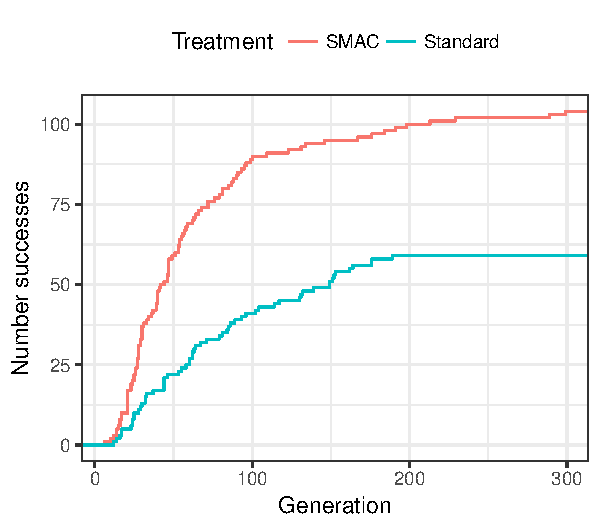
\includegraphics[width=3in]{../figures/successGenerations}
	\caption{Cumulative success counts over time for both the Standard
	and the SMAC parameter settings.}
	\label{fig:successGenerations}
\end{figure}

As Figure~\ref{fig:successGenerations} illustrates, the runs using the SMAC
parameter configuration also discovered solutions much earlier than runs using
the Standard parameters. By generation 100, for example, 90 of the 110 SMAC 
runs (or 87\%) had succeeded, where only 41 of the 110 Standard runs 
(or 37\%) had succeeded. All the pairwise (by generation) differences 
between SMAC and Standard cumulative counts in 
Figure~\ref{fig:successGenerations} are 
statistically significant ($p<0.015$)
from generation 29 forward.\footnote{Using a $\chi^2$ test of proportions 
	with the Holm correction for the 300 separate comparisons.}

\subsection{Impact of SMAC parameters on RSWN}
\label{sec:SMACimpactRSWN}

\todo{Document impact on distribution of operators in ancestry graphs.}

A key change from the Standard parameter settings to the SMAC parameters
are the changes in the genetic operator probabilities, as outlined in
Table~\ref{table:results}. A question this then raises is how these changes
actually impact the dynamics of the resulting runs, and in particular if and
how they affect the likelihood of a given genetic operator playing a key
role in the ultimate discovery of a solution.

\begin{figure*}
	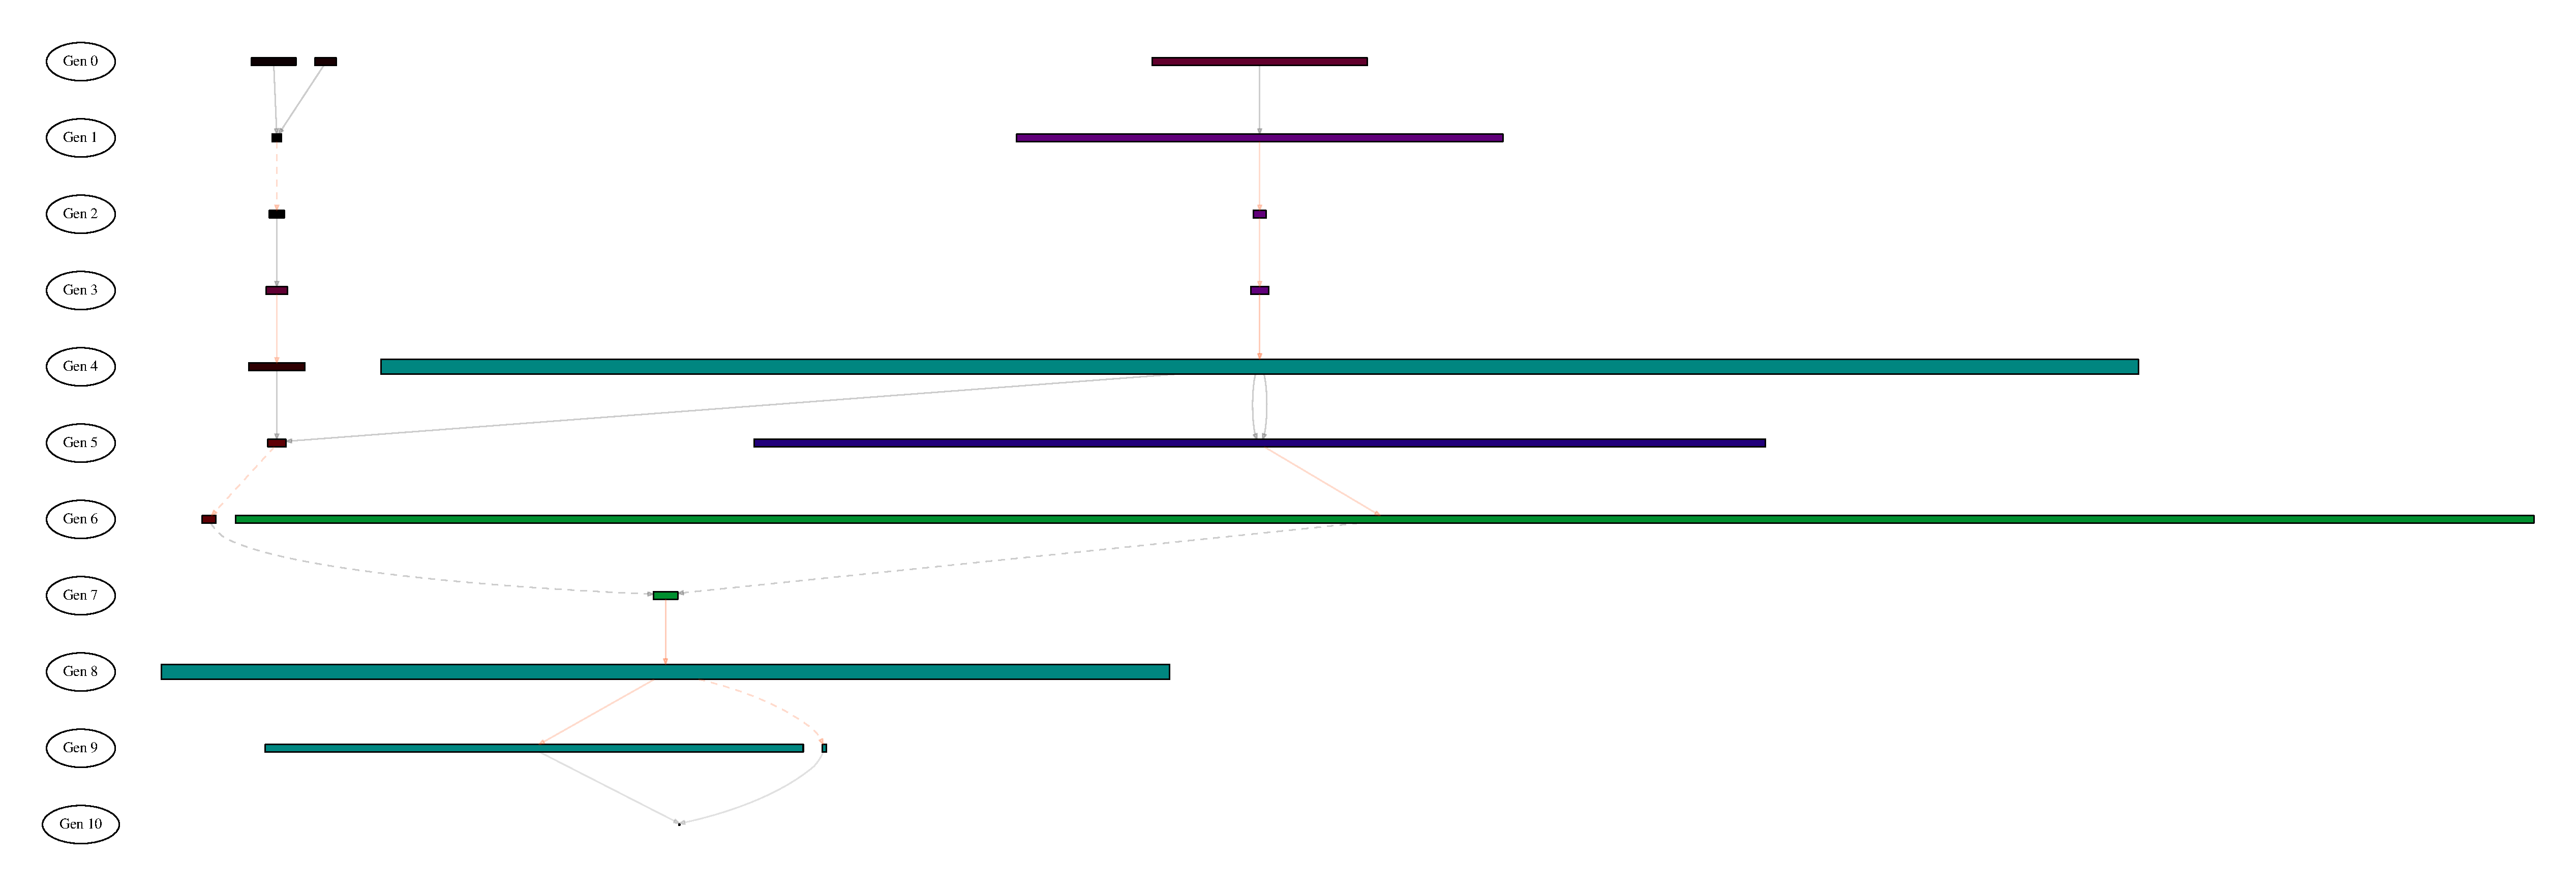
\includegraphics[width=6in]{../figures/log1_filter_by_genes_vanilla}
	\caption{Ancestry graph of a successful Replace-space-by-newline run
	using the ``tuned'' parameters discovered by SMAC. This tree is filtered 
	to only include individuals that ultimately passed a gene
	on to the winning individual.}
	\label{fig:log1ByGenes}
\end{figure*}

To address this question, we did 10 runs of Replace-space-with-newline (RSWN) 
using the Standard parameters and 10 using the SMAC parameters, 
collecting highly detailed records of parent-child relationships 
among individuals, as well as information on which genes in the Plush 
genomes of parents were copied into
the genomes of their children. This allowed us to compute full ancestry
graphs for 
runs~\cite{McPhee:2016:VGP:2908961.2931741,McPhee:2015:GPTP,McPhee:2016:GPTP},
tracing back from the ``winning'' individuals (programs that have zero error)
to discover all their ancestors. Figure~\ref{fig:log1ByGenes}, for example,
shows the ancestry graph for one successful RSWN run using the SMAC parameters.
\todo{We should replace this graph with one with a more sensible shaping (e.g., width proportional to the number of genes passed to the child). We may also
want to have two graphs, one filtered and one not filtered to illustrate those
two approaches.}

\todo{Explain that we collected operator counts in the three different subsets
	of the entire collection of individuals, and then plot those, and then
	try to make some sense of the plot.}

\section{Applying those parameters to other problems}
\label{sec:applyingToOtherProblems}

%These are the parameters I'm using, which are approximately those taken from Nic's SMAC optimizations on RSWN:
%
%\begin{verbatim}
%:uniform-mutation-rate 0.18
%:alignment-deviation 120
%:genetic-operator-probabilities {:alternation 0.04
%                                 :uniform-mutation 0.36
%                                 :uniform-close-mutation 0.06
%                                 [:alternation :uniform-mutation] 0.54}
%\end{verbatim}
%
%All other pushgp parameters are set to default, including population size of 1000.

\begin{table}[t]
\centering
\caption{Number of successful programs out of 100 runs with standard parameters (those in the ``Default'' column of Table~\ref{tab:clojushParameters}), and with the parameters that SMAC found when run on RSWN.}
\label{table:results}
%\rowcolors{3}{Gray}{white}
\begin{tabular}{l r r}
\toprule
\textbf{Problem} & \textbf{Standard Params} & \textbf{SMAC Params} \tabularnewline
\midrule
\textit{Replace Space with Newline} & \textit{54} & \textit{91} \tabularnewline
Double Letters	& 0 & 6 \tabularnewline
String Lengths Backwards & 68 & 75 \tabularnewline
Syllables & 22 & 17 \tabularnewline
X-Word Lines & 17 & 3 \tabularnewline
\bottomrule
\end{tabular}
\end{table}

One of the hopes of using SMAC is that parameters found when optimizing one problem might be transferable to other problems with similar requirements. To test whether the parameters we found with SMAC on RSWN can be helpful for other problems, we conducted sets of 100 runs on 4 other problems from the same program synthesis benchmark suite: Double Letters, Stirng Lengths Backwards, Syllables, and X-Word Lines. Each of these problems requires a solution program that manipulates strings like RSWN, but otherwise has different requirements. For example, the Syllables problem requires the program to count the number of vowels in a given input string.

In Table~\ref{table:results} we present the number of successful runs out of 100 for each problem, using both the default parameters and those found with SMAC on RSWN. Note that we only count a program as a success if it generalizes to an unseen set of test data. Of these results, the SMAC parameters are only significantly better on the Double Letters problem.\footnote{Using a $\chi^2$ test of proportions with a significance level of $0.05$.} 
Conversely, SMAC's settings gave significantly worse resutls on the X-Word Lines problem, and no significant difference on the other two problems.

These results indicate that while the parameters discovered by SMAC on RSWN do significantly improve results on RSWN itself, they do not provide any improvements on other similar problems. This leads to the conclusion that there is some characteristic of the RSWN problem that makes high mutation rates and high alignment deviations able to find solutions much more quickly, and that this characteristic does not hold for other similar types of problems


\section{Discussion}
\label{sec:discussion}

Talk about what we learned and what this means

A piece from @thelmuth at Discourse that we might want to use:
\begin{quote}
	Here's a simpler version of my first explanation: alternation makes viable children more often, so you need less of it per event that you want to be successful. Uniform mutation makes viable children less often, so you need more of it per event that you want to be successful. Uniform close mutation makes viable children the most often, so you need least of it per event you want to be successful. Then, in the ancestors of the solution, you get the percents of the events you want to be successful, not the percent of the events you have in total.
\end{quote}

\section{Future work}
\label{sec:futureWork}

\begin{itemize}
	\item Use SMAC to tune parameters on the other four problems one at a time, and see how that works on the other problems.
	\item Use SMAC to tune on (sub)sets of the problems, like all 5, or on subsets that seem similar (or different) based on the individual tuning.
	\item etc.
\end{itemize}

\section{Conclusions}
\label{sec:conclusion}

Evolution is complicated!

